% !TEX TS-program = pdflatex
% !TEX encoding = UTF-8 Unicode

% This is a simple template for a LaTeX document using the "article" class.
% See "book", "report", "letter" for other types of document.

\documentclass[11pt]{article} % use larger type; default would be 10pt

\usepackage[utf8]{inputenc} % set input encoding (not needed with XeLaTeX)

%%% Examples of Article customizations
% These packages are optional, depending whether you want the features they provide.
% See the LaTeX Companion or other references for full information.

%%% PAGE DIMENSIONS
\usepackage{geometry} % to change the page dimensions
\geometry{letterpaper} % or letterpaper (US) or a5paper or....
\geometry{margin=1in} % for example, change the margins to 2 inches all round
% \geometry{landscape} % set up the page for landscape
%   read geometry.pdf for detailed page layout information

\usepackage{graphicx} % support the \includegraphics command and options
\usepackage{colortbl}
% \usepackage[parfill]{parskip} % Activate to begin paragraphs with an empty line rather than an indent
\usepackage{amssymb}
\usepackage{amsmath}
\usepackage{amsfonts}
\usepackage{bbm}
\usepackage{amsthm}

%%% PACKAGES
\usepackage{booktabs} % for much better looking tables
\usepackage{array} % for better arrays (eg matrices) in maths
\usepackage{paralist} % very flexible & customisable lists (eg. enumerate/itemize, etc.)
\usepackage{verbatim} % adds environment for commenting out blocks of text & for better verbatim
\usepackage{subfig} % make it possible to include more than one captioned figure/table in a single float
% These packages are all incorporated in the memoir class to one degree or another...

%%% HEADERS & FOOTERS
\usepackage{fancyhdr} % This should be set AFTER setting up the page geometry
\pagestyle{fancy} % options: empty , plain , fancy
\renewcommand{\headrulewidth}{0pt} % customise the layout...
\lhead{}\chead{}\rhead{}
\lfoot{}\cfoot{\thepage}\rfoot{}

%%% SECTION TITLE APPEARANCE
\usepackage{sectsty}
\allsectionsfont{\sffamily\mdseries\upshape} % (See the fntguide.pdf for font help)
% (This matches ConTeXt defaults)

%%% ToC (table of contents) APPEARANCE
\usepackage[nottoc,notlof,notlot]{tocbibind} % Put the bibliography in the ToC
\usepackage[titles,subfigure]{tocloft} % Alter the style of the Table of Contents
\usepackage{bbm}
\usepackage{endnotes}
\renewcommand{\qed}{\hfill\blacksquare}
\renewcommand{\cftsecfont}{\rmfamily\mdseries\upshape}
\renewcommand{\cftsecpagefont}{\rmfamily\mdseries\upshape} % No bold!
\DeclareMathOperator*{\argmax}{arg\,max}
\DeclareMathOperator*{\argmin}{arg\,min}
\usepackage{graphicx}
\graphicspath{ {./pings/} }

\newcount\colveccount
\newcommand*\colvec[1]{
	\global\colveccount#1
	\begin{pmatrix}
		\colvecnext
	}
	\def\colvecnext#1{
		#1
		\global\advance\colveccount-1
		\ifnum\colveccount>0
		\\
		\expandafter\colvecnext
		\else
	\end{pmatrix}
	\fi
}

\newcommand{\norm}[1]{\left\lVert#1\right\rVert}

\title{Problem Set \#6\\ ~\\ \large{Econ 899, Fall 2021} }
\author{Heejin Yoon}


\begin{document}
\maketitle
~\\

\section*{Tasks 1 and 2}
\begin{itemize}
	\item[] Both versions of the Hopenhayn and Rogerson (1993) model are calculated, and the results are presented below.
	
	\begin{center}
	\begin{tabular}{c|c|c|c} 
		\hline\hline
		\textbf{Variable}             & \textbf{Standard} & \textbf{TV1 Shock ($\alpha=1$)} & \textbf{TV1 Shock ($\alpha=2$)}  \\ 
		\hline\hline
		Price Level                   & 0.739             & 0.691                                            & 0.719                                             \\
		Mass of Incumbents            & 6.66              & 6.74                                             & 6.04                                              \\
		Mass of Entrants              & 1.66              & 2.81                                             & 2.31                                              \\
		Mass of Exits                 & 2.64              & 4.22                                             & 3.51                                              \\
		Aggregate Labor               & 179.83            & 188.89                                           & 182.62                                            \\
		Labor of Incumbents           & 142.63            & 139.50                                           & 136.65                                            \\
		Labor of Entrants             & 37.20             & 49.39                                            & 45.97                                             \\
		Fraction of Labor in Entrants & .207              & .261                                             & .252                                              \\
		\hline\hline
	\end{tabular}
	\end{center}
	
	\item[] With randam disturbances, the price level drops and a change in price makes the mass of entrants increase. This, in turn, positively affects the mass of incumbents, as well as the mass of exits. 
\end{itemize}
	\pagebreak


\section*{Task3}
\begin{itemize}
	\item[] The decision rules of exit is illustrated below. With random shocks, the least productive firms do not exit with certainty, and there exists some probability that the second least productive firms exit. Nevertheless, there still is a negative correlation between the productivity of firms and the probability of exit.
	
	\begin{center}
	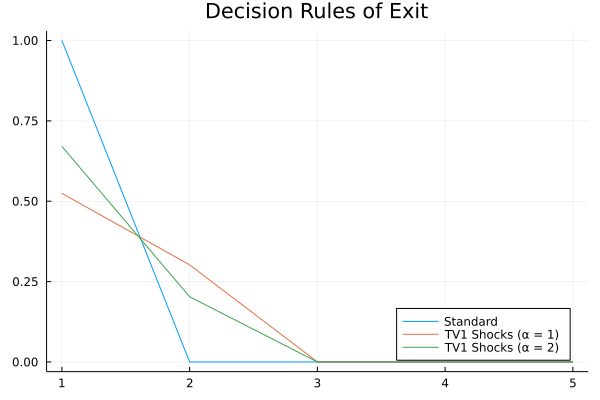
\includegraphics[width=.8\linewidth]{./exit_func1.png}
	\end{center}	
\end{itemize}
	\pagebreak
	
\section*{Task4}
\begin{itemize}
	\item[] If we increase fixed costs to $15$, then the second least productive firms exit with certainty in the standard model. Random shocks alleviates this obvious relationshp, but in TV1 shock with $\alpha=1$ the least productive firms almosty certainly exits.
	
	\begin{center}
		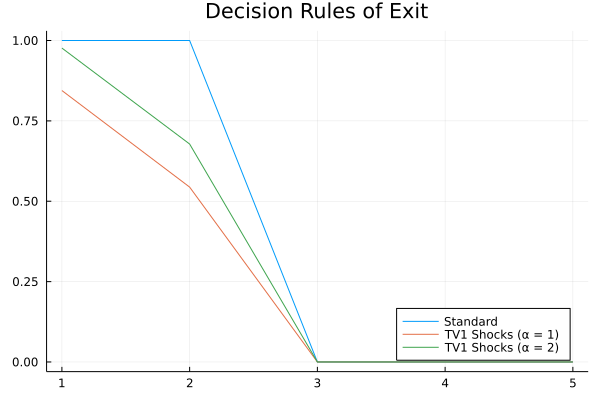
\includegraphics[width=.8\linewidth]{./exit_func2.png}
	\end{center}
	
\end{itemize}
	
\end{document}